\documentclass[11pt]{article}
\usepackage{fullpage}
\usepackage{mathtools}
\usepackage{pdfpages}

\begin{document}

\title{Praktikumsbericht\\ Resonanzverhalten eines Masse-Federsystems (M10)\\24.01.2019}
\author{Gruppe C8, Janosch Ehlers, Tobias Buchmann}
\maketitle

\begin{center}
\textsc{Inhalt}
\end{center}
\begin{enumerate}
\item Ziel des Versuchs
\item Theoretischer Hintergrund
\item Versuchsaufbau und -durchführung
\item Auswertung
\item Anhang
\end{enumerate}

\section{Ziel des Versuchs}
Untersucht werden hier freie, freie gedämpfte und erzwungene Schwingungen bei Masse-Feder Systemen. Dabei werden die von CASSY aufgezeichneten Resonanzkurven ausgewertet. In mehreren Versuchen wurden nun die Eigenfrequenzen von verschiedenen Systemen untersucht. Außerdem wurden über zwei Ansätze die Dämpfungskonstante untersucht und verglichen.

\section{Theoretischer Hintergrund}
Diesem Experiment zugrunde liegt ein die Kombination aus dem 2. Newtonschen Axiom und dem hookschen Gesetz nach: $$m\frac{d^2x}{dt^2}+Dx=0$$ Dies hat eine Lösung: $$\omega_0=2\pi f_0=\frac{2\pi}{T_0}=\sqrt{\frac{D}{m}}$$ und gilt für freie ungedämpfte harmonische Schwingungen. Für gedämpfte harmonische Schwingungen muss ein Dämpfungsfaktor hinzugefügt werden. Dieser ist hier $B$ und wir der Differenzialgleichung als Summand hinzugefügt:$$m\frac{d^2x}{dt^2}+B\frac{dx}{dt}+Dx=0$$ Für schwache Dämpfung ($B^2\leq4Dm$) kann die Gleichung wie folgt gelöst werden:$$\omega_1=2\pi f_1=\frac{2\pi}{T_1}=\sqrt{\frac{D}{m}-\frac{B^2}{4m^2}}$$ Weiterhin wichtig ist das Dämpfungsverhältnis. Dieses gibt über: $$\frac{x_n}{x_{n-1}}=\exp(\frac{BT_1}{2m})=\exp(\delta T_1)$$ Auskunft über die Dämpfungskonstante $\delta$. Der nächste Schritt zur Berechnung dieser ist der natürliche Logarithmus der Gleichung: $$\Lambda=\ln\frac{x_n}{x_{n-1}}=\frac{BT_1}{2m}=\delta T_1$$ dieser Ausdruck wird logarithmisches Dekrement($\Lambda$) genannt. Ein weiterer Ansatz die Dämpfungskonstante zu berechnen ist die Abtragung der Amplitude bei einer erzwungenen Schwingung. Die daraus resultierende Glockenkurve kann dann über die eigene Halbwertsbreite ausgewertet werden. Die Halbwertsbreite:= HWB. Dabei gilt: $HWB = 2\cdot\Delta\omega$ während $\Delta\omega\approx\delta\sqrt{3}$ gilt.

\section{Versuchsaufbau und -durchführung}
Aufgebaut ist ein Massestück, welches über zwei Federn befestigt ist. Die obere Feder ist an ein digitales Kraftmessgerät fixiert. Die untere Feder hingegen ist an eine Schubstange befestigt, welche durch eine Spule bewegt werden kann. Die Daten des Kraftmessers werden von dem Computerprogramm CASSY aufgezeichnet. Die Spule ist über ein Ampermeter an ein Frequenzgenerator angeschlossen. Die vom Frequenzgenerator erzeugte Schwingung kann die Schubstange in Schwingung versetzen. Das Massestück wird dadurch in eine sogenannte erzwungene Schwingung versetzt. Ein Schema des gesamten Aufbaus ist im Anhang unter Diagramm 3 zu finden. An das Massestück ist ein Magnet befestigt. Wird eine Aluminiumröhre um das Massestück befestigt, erzeugt der Magnet in der Röhre eine Gegenbeschleunigung, ähnlich der Funktionsweise einer Wirbelstrombremse. Dies ist wichtig für die Untersuchung einer gedämpften Schwingung.

\section{Auswertung}
 
Bestimmung der Eigenfrequenz der freien Schwingung $\omega_0$ aus der gemessenen Frequenz $f_0$:\\
$$\omega_0= 2\pi\cdot f_0$$ 
\begin{center}
$f_0=(1,690\pm 0,001)Hz$\\
$\omega_0=(10,619\pm 0,006)\frac{1}{s}$\\
\end{center}

Bestimmung der Eigenfrequenz der freien gedämpften Schwingung:\\
\begin{center}
$f_1 =(1,692\pm 0,001)Hz$\\
$\omega_1=(10,631\pm 0,006)\frac{1}{s}$\\
\end{center}

Bestimmung der Dämpfungskonstante B aus der Abklingkonstante $\delta$ und der Masse $m$ für die freie gedämpfte Schwingung mittels Anpassung der Einhüllenden:\\
\begin{center}
$\delta=0,212 \frac{1}{s}$\\
$m=(0,0568\pm 0,0001)kg$
$$\delta=\frac{B}{2m} \Leftrightarrow B = \delta 2m$$
$B=(0,02407\pm 0,00004) \frac{Kg}{s}$\\
\end{center}

Aus der aufgenommenen Resonanzkurve wurde eine Halbwertsbreite HWB von $(0,081\pm 0,001)\frac{1}{s}$ bestimmt. Daraus lässt sich die Dämpfungskonstante $\delta$ bestimmen mit:
\begin{center}
$$HWB=2\Delta\omega$$
$$\Delta\omega = \delta*\sqrt{3}$$
$\Delta\omega=(0,0405\pm 0,0005)\frac{1}{s}$\\
$\delta=(0,0234\pm 0,0003)\frac{Kg}{s}$\\
\end{center}

Die beiden auf verschiedenen Wegen bestimmten Dämpfungskonstanten liegen sehr nah beieinander, was nahelegt, dass beide Arten der Bestimmung der Dämpfungskonstanten gut geeignet sind. Die Fehler der Messinstrumente haben dabei nur geringen Einfluss auf die erhaltenen Werte. Der größte Fehler liegt in der grafischen Bestimmung aus der Resonanzkurve, da die subjektive Einschätzung der Lage der Resonanzkurve und der damit bestimmten Halbwertsbreite signifikant die Dämpfungskonstante beeinflusst.  

\section{Anhang}

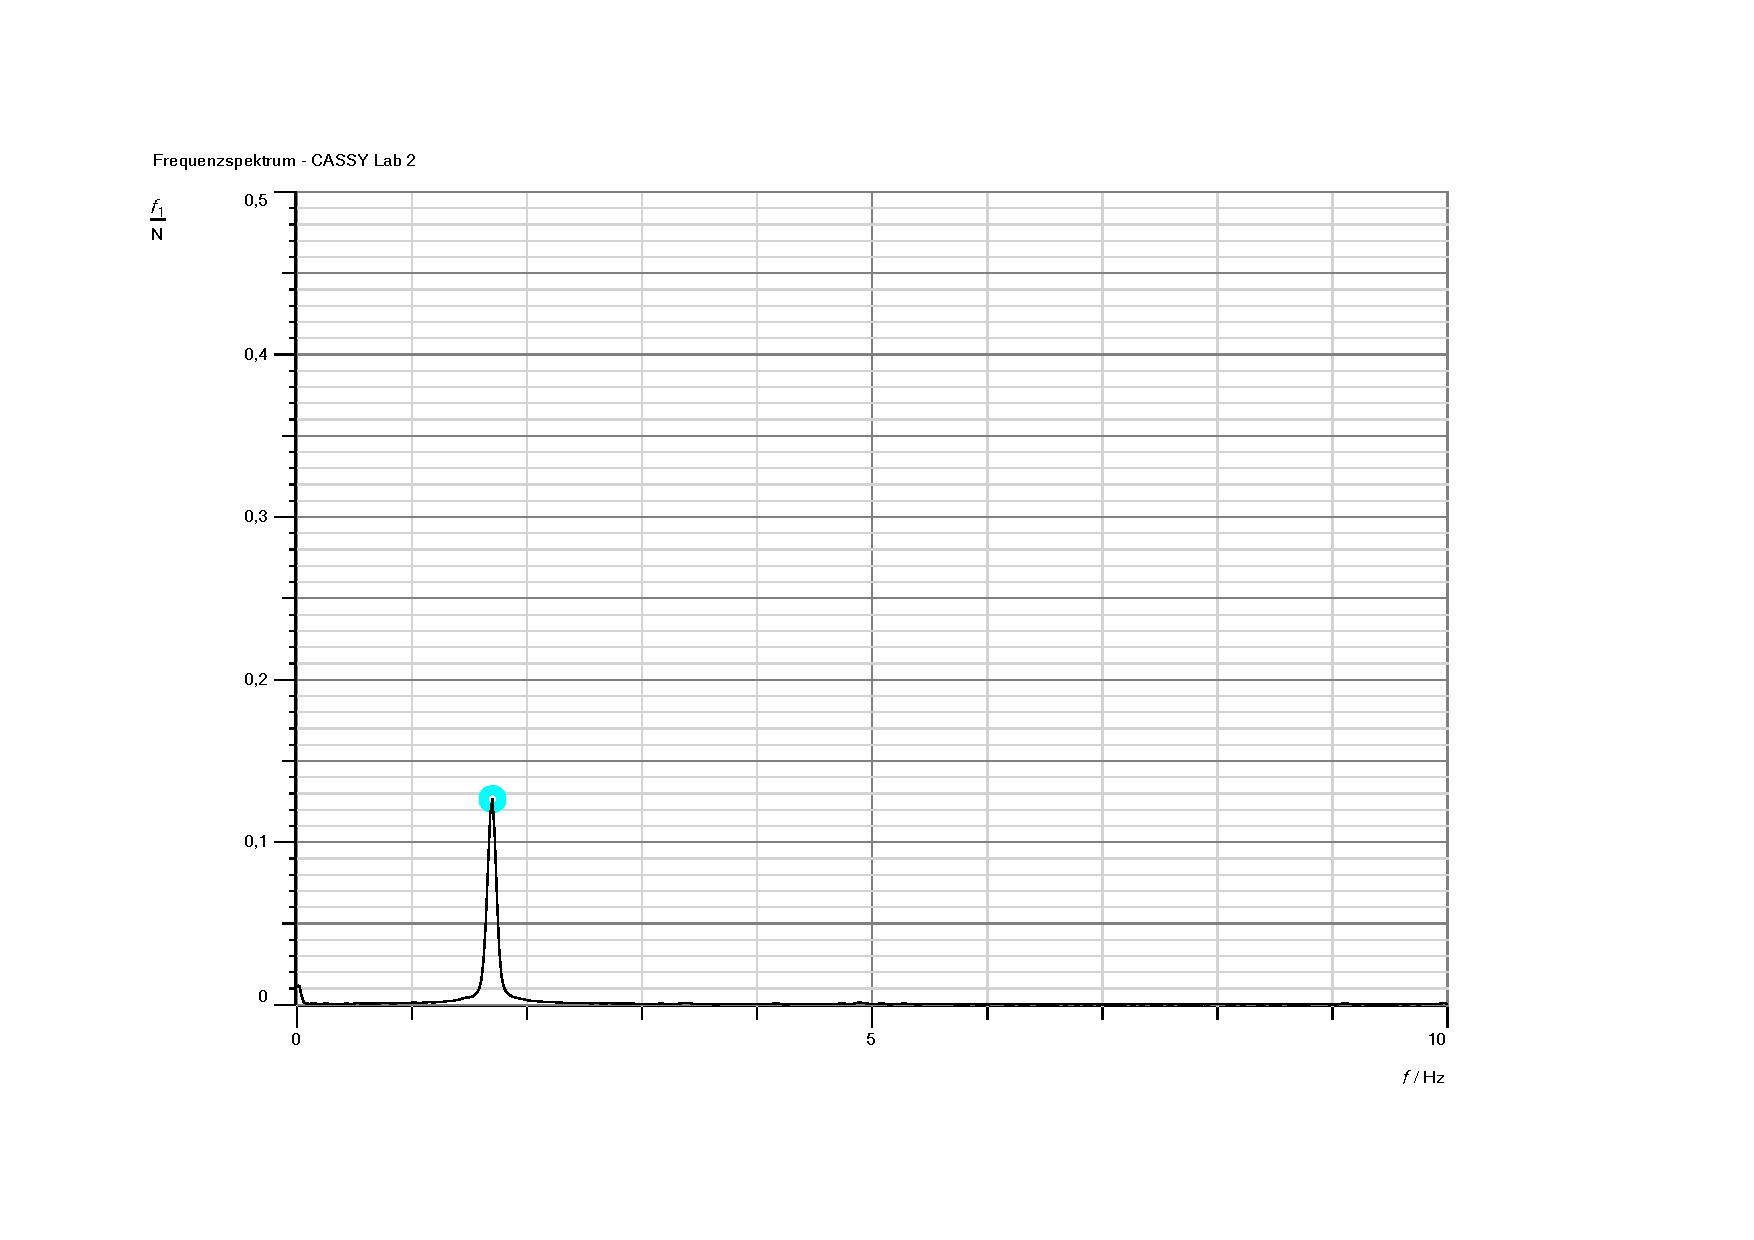
\includepdf[angle=270]{./Frequenzspektrum.pdf}
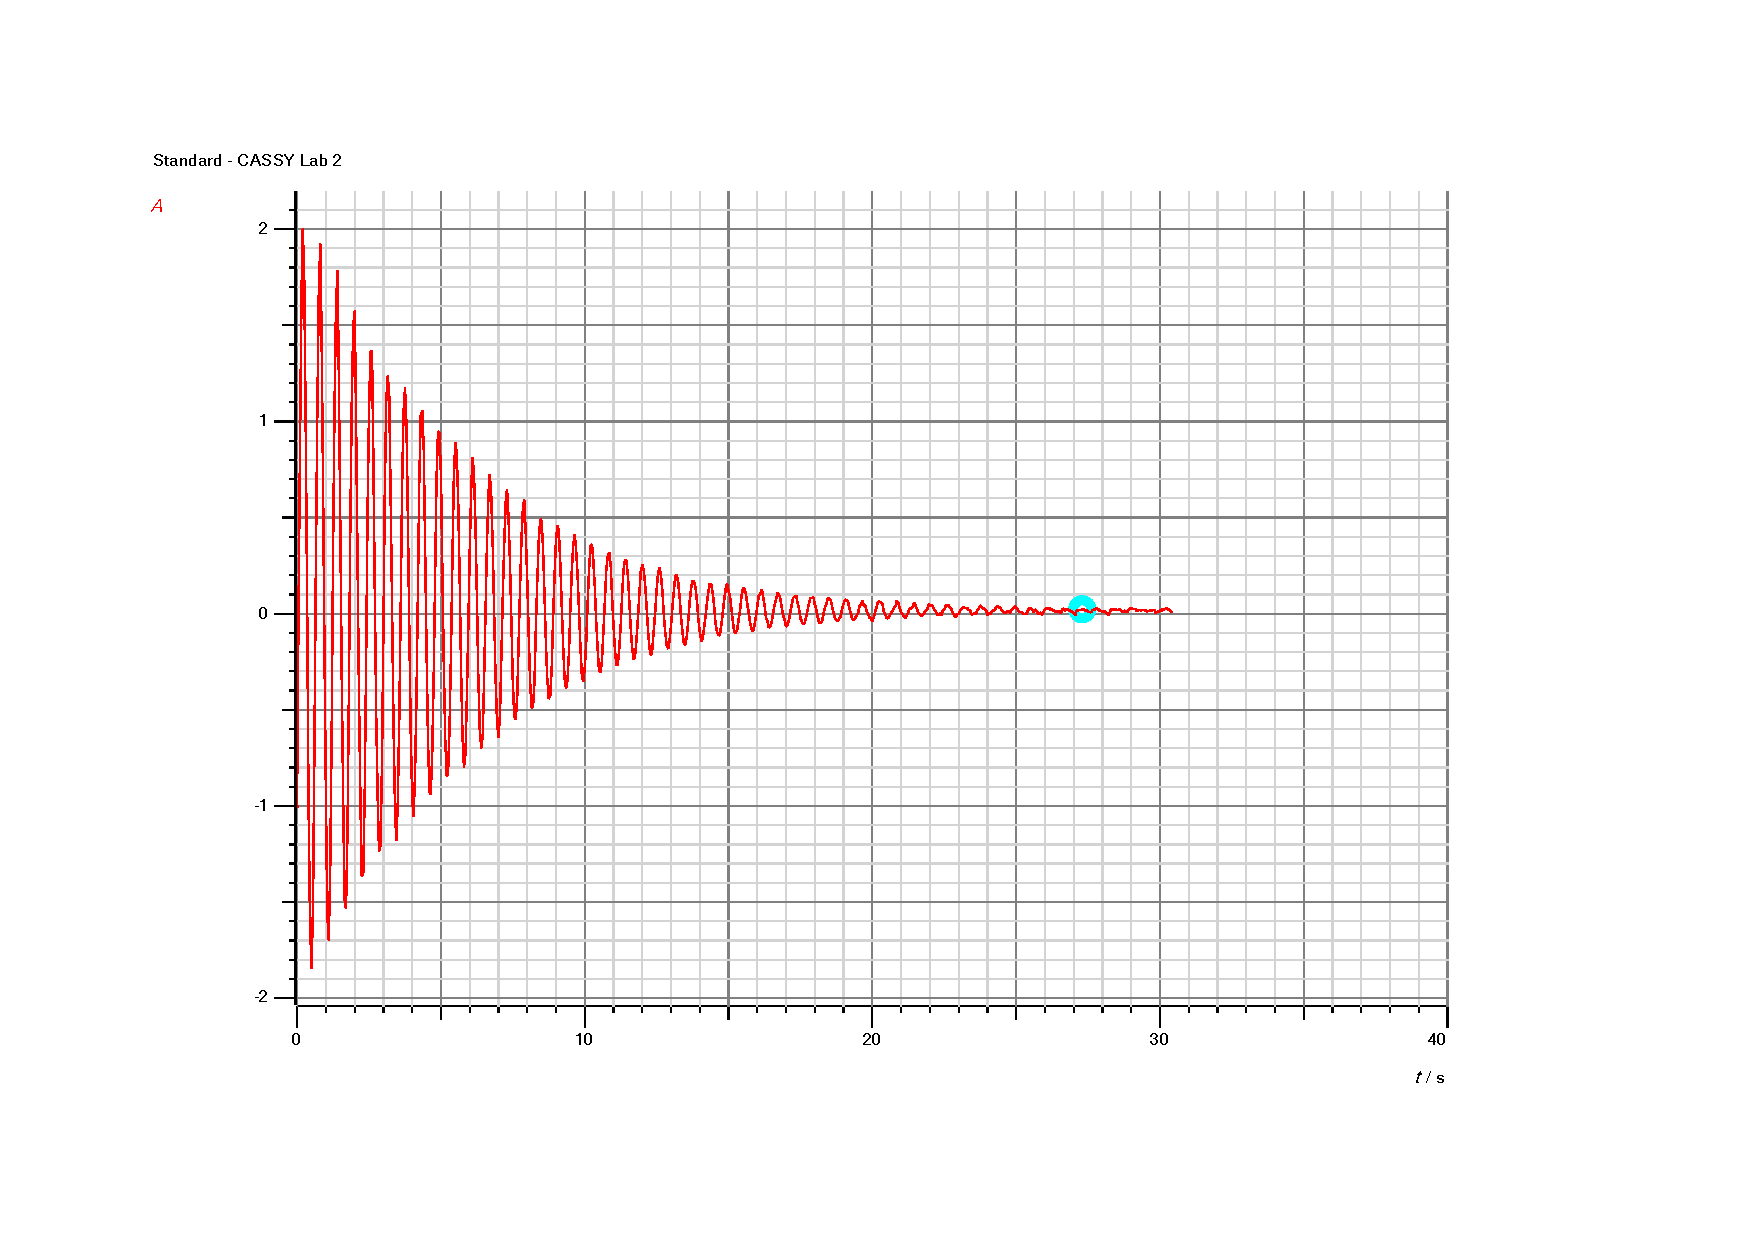
\includepdf[angle=270]{./GedaempfteSchwingung.pdf}
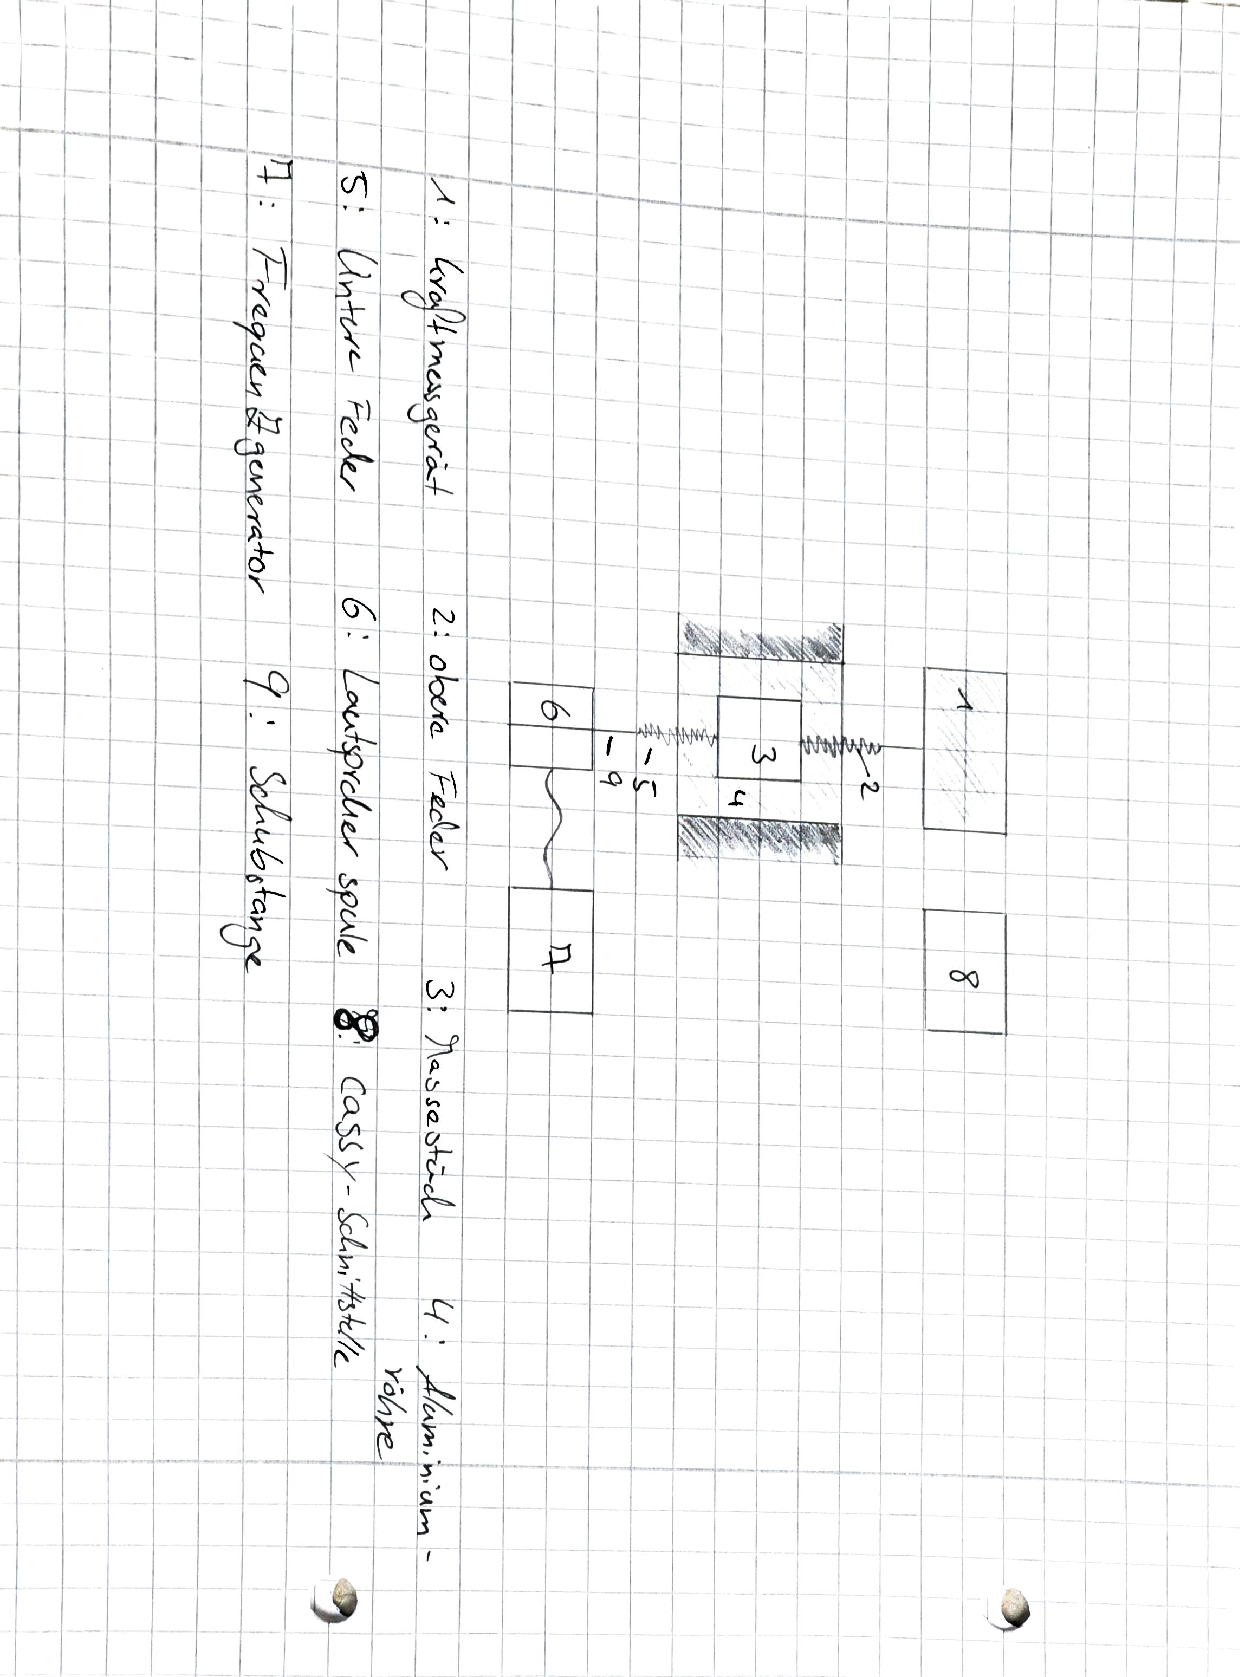
\includepdf[]{./Aufbau.pdf}
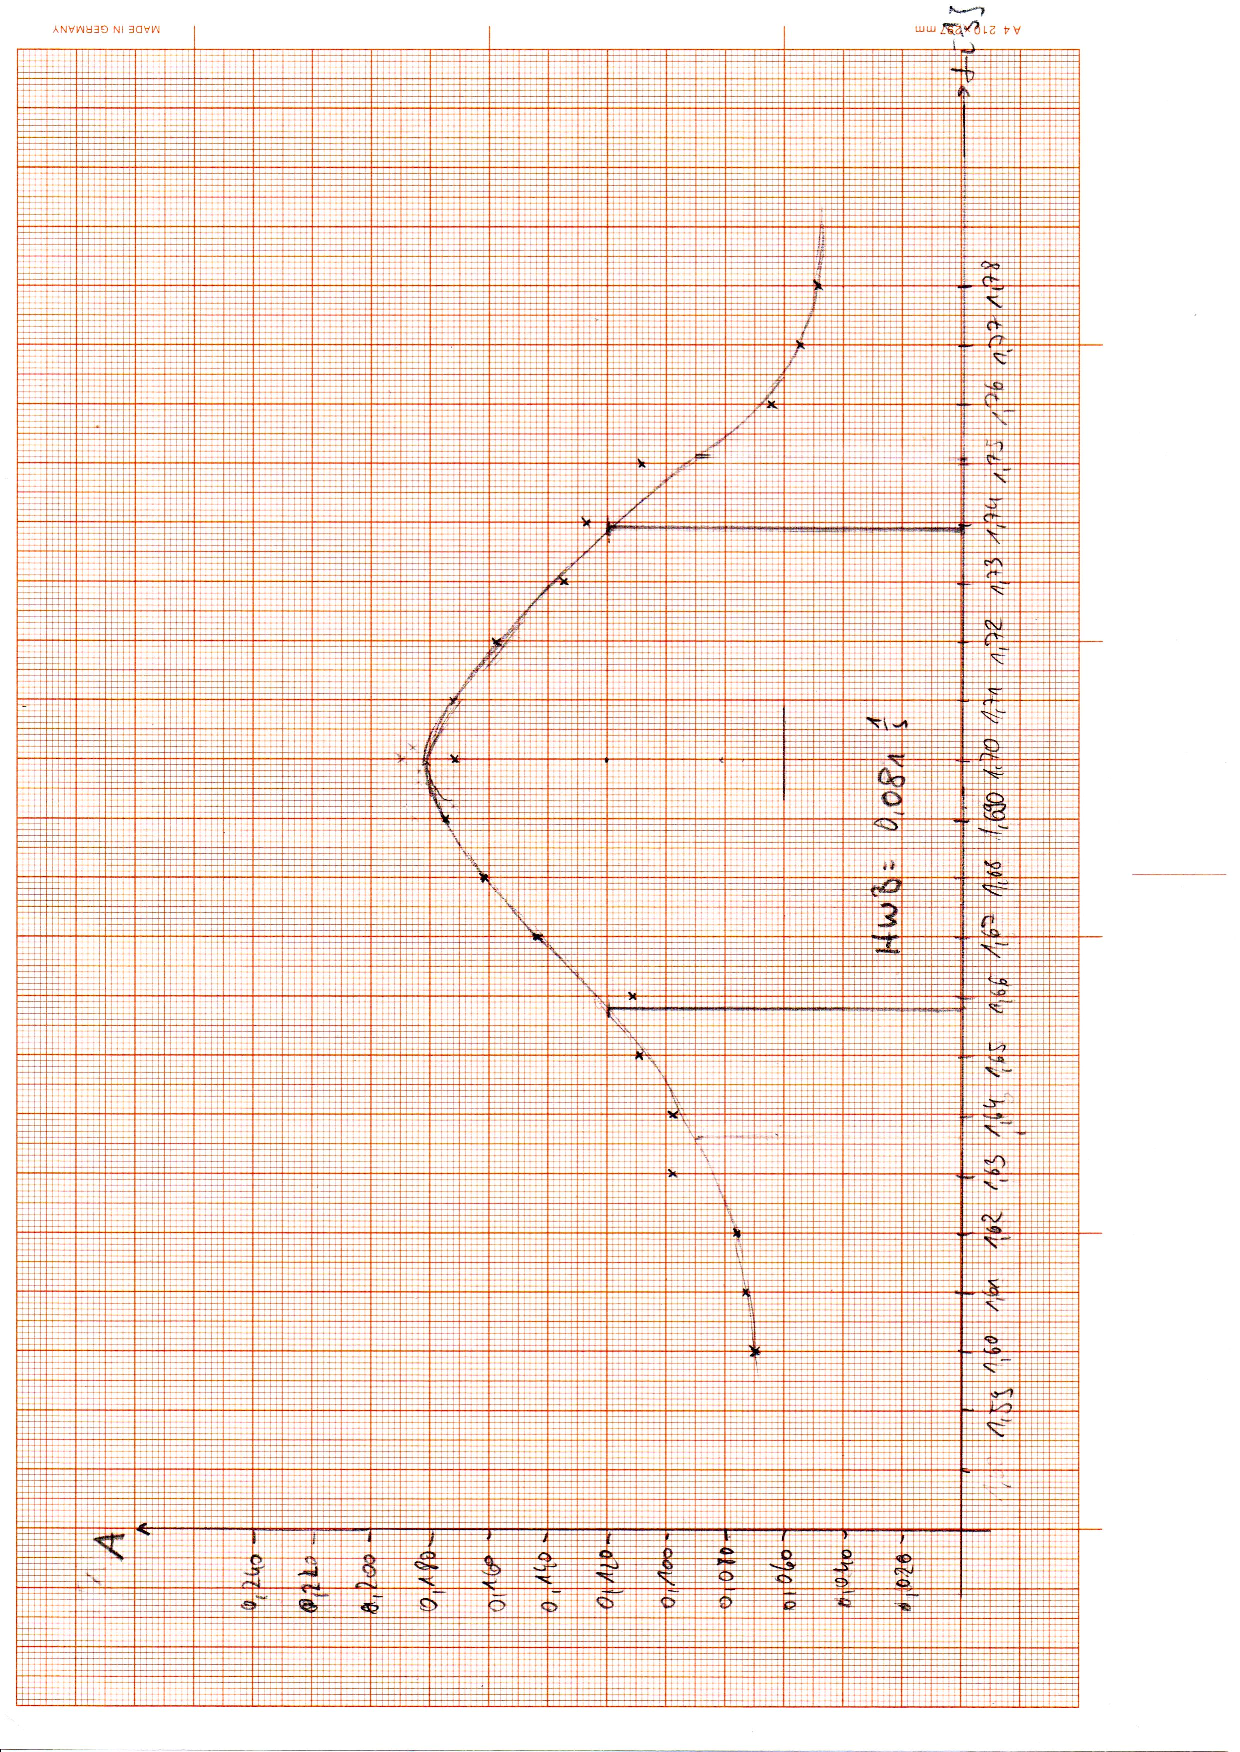
\includepdf[angle=180]{./Messdaten_Glockenkurve.pdf}

\end{document}
